After the integration tests of each bending operation, the program for each bending stage is compiled together to create a main program which cycles through all bending operations for the test sheet metal part. After all six bending operations on the test part, \hyperref[acro:KR]{KR1410} robot loads the sheet in the drawer of storage station.
The main program is based on the flowchart \ref{tab:flowchart} and uses the variables shared with the \hyperref[acro:PLC]{PLC} (as shown in table \ref{tab:kr1410-to-plc} and \ref{tab:plc-to-kr1410}) to perform the bending.

A cycle starts when a new sheet is requested by the \hyperref[acro:KR]{KR1410}. It ends with the placement of bent sheet in the drawer of the shelf. After all the optimizations for trajectory planning in teach pendant, the cycle time comes out to be around \textbf{4 minutes and 10 seconds} with all inspection jobs. Without any inspection, the cycle time reduces to 3 minutes and 40 seconds. An inspection is not done for all parts. After every five parts, one part is selected for inspection. This is done in order to reduce the production time.

The performance of the bending process is evaluated in the following sections using the calibration results, inspection assessment and reviewing the bending operation.

\section{Calibration Results}
\label{sec:calibration-results}
Calibration is fundamental to ensuring the accuracy and reliability of an automated robotic workcell. The calibration process takes exactly 98 seconds for the robot. Proper calibration ensures that the robot operate with high accuracy, thus reducing variability in the bent sheet metal part.

Figure \ref{fig:calibration-parameters} shows the calibration parameters after an automatic calibration. The field of view is 100\% with a resolution of 0.1564 mm/pixel.

\begin{figure}[h]
    \centering
    \begin{subfigure}{0.48\textwidth}
        \centering
        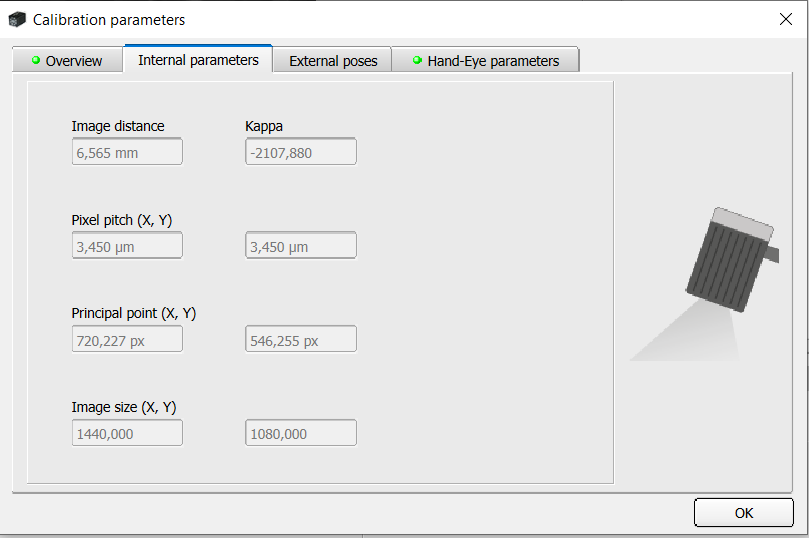
\includegraphics[width=\textwidth]{figures/001calibration/internal_parameters.PNG}
        \caption{Internal parameters}
        \label{subfig:internal-parameters}
    \end{subfigure}\hspace{0cm}
    \begin{subfigure}{0.48\textwidth}
        \centering
        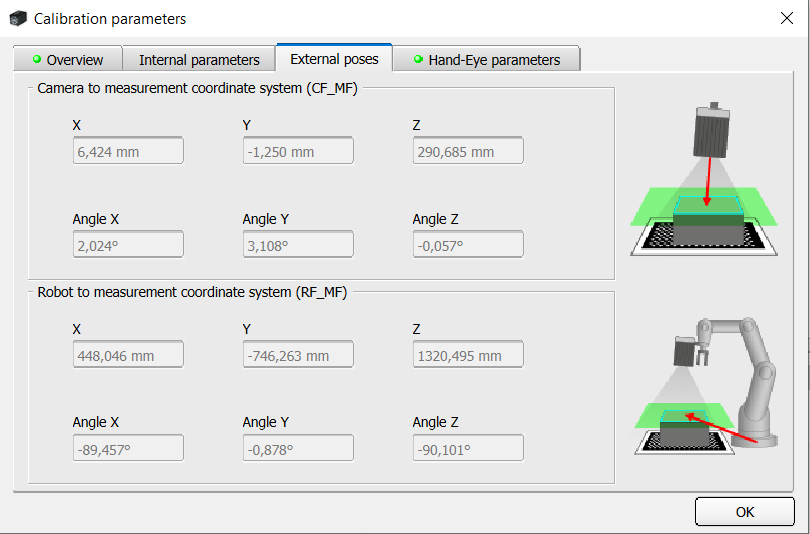
\includegraphics[width=\textwidth]{figures/001calibration/external_poses.PNG}
        \caption{External poses}
        \label{subfig:external-poses}
    \end{subfigure}
    \begin{subfigure}{0.48\textwidth}
        \centering
        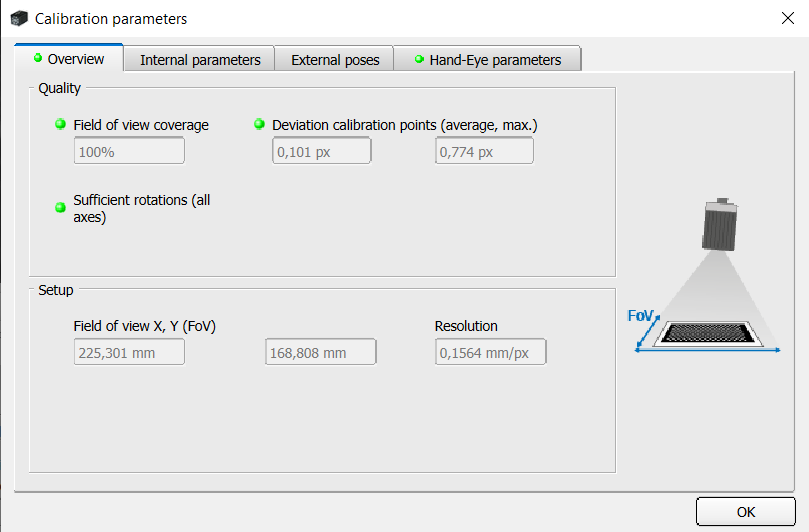
\includegraphics[width=\textwidth]{figures/001calibration/fov.PNG}
        \caption{Field of view}
        \label{subfig:fov}
    \end{subfigure}
    \begin{subfigure}{0.48\textwidth}
        \centering
        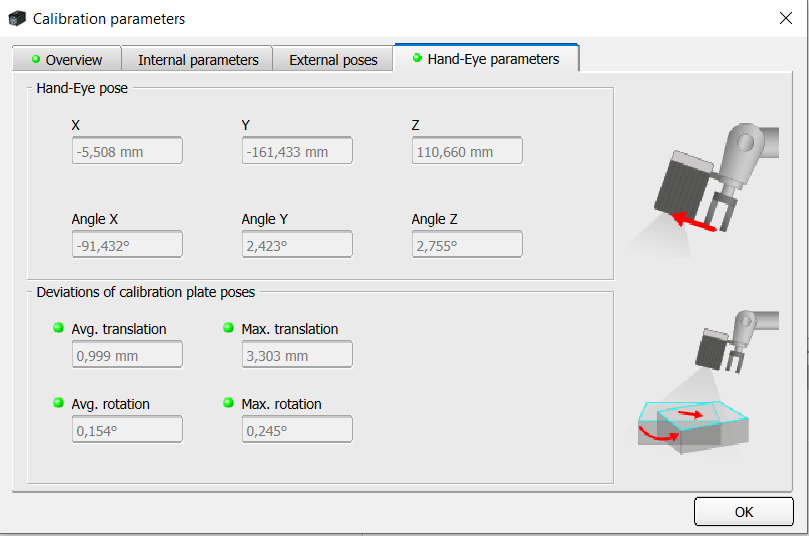
\includegraphics[width=\textwidth]{figures/001calibration/hand-eye_parameters.PNG}
        \caption{Hand-eye parameters}
        \label{subfig:hand-eye-parameters}
    \end{subfigure}
    \caption{Calibration parameters}
    \label{fig:calibration-parameters}
\end{figure}


By establishing rigorous calibration procedures, the automated robotic workcell can achieve optimal performance, ensuring that the bending process is executed with high precision and reliability.  The \hyperref[acro:KR]{KR1410} robot only has a repeatability of 0.1 mm. After the \hyperref[acro:TCP]{TCP} calibration, the bending process has a repeatability of 0.5 mm, which is still better than a human operator.

\FloatBarrier  % Force all figures of the first section to be placed before the next section

\section{Inspection Assessment}
\label{sec:inspection-assessment}
The inspection of only four bending operations out of six bendings are required for the test part. Figure \ref{fig:bending-inspection} shows these inspection camera images upon trigger. Figure \ref{subfig:inspection-1}, \ref{subfig:inspection-5} and \ref{subfig:inspection-6} tests the bending operation of 90\textdegree which is performed at bending station 1. Figure \ref{subfig:inspection-2} is the testing of bending of 135\textdegree which happens at bending station 2.

Table \ref{tab:bending-data} shows the bending angles as measured by the inspection camera for ten sheet metal parts. The angle measurement is pretty close to each other. The angle is measured by the light reflected by the edge of sheet metal part. Because of different surface roughness and impurities on surface, there is slight deviation in the bending angles measured. A tolerance of 90$\pm5$\textdegree{} is set for the bending 1, bending 5 and bending 6. For bending 2, a tolerance of 135$\pm10$\textdegree{} is set. These tolerance values can be adjusted on the SIMATIC HMI.

\begin{figure}[h]
    \centering
    \begin{subfigure}{0.48\textwidth}
        \centering
        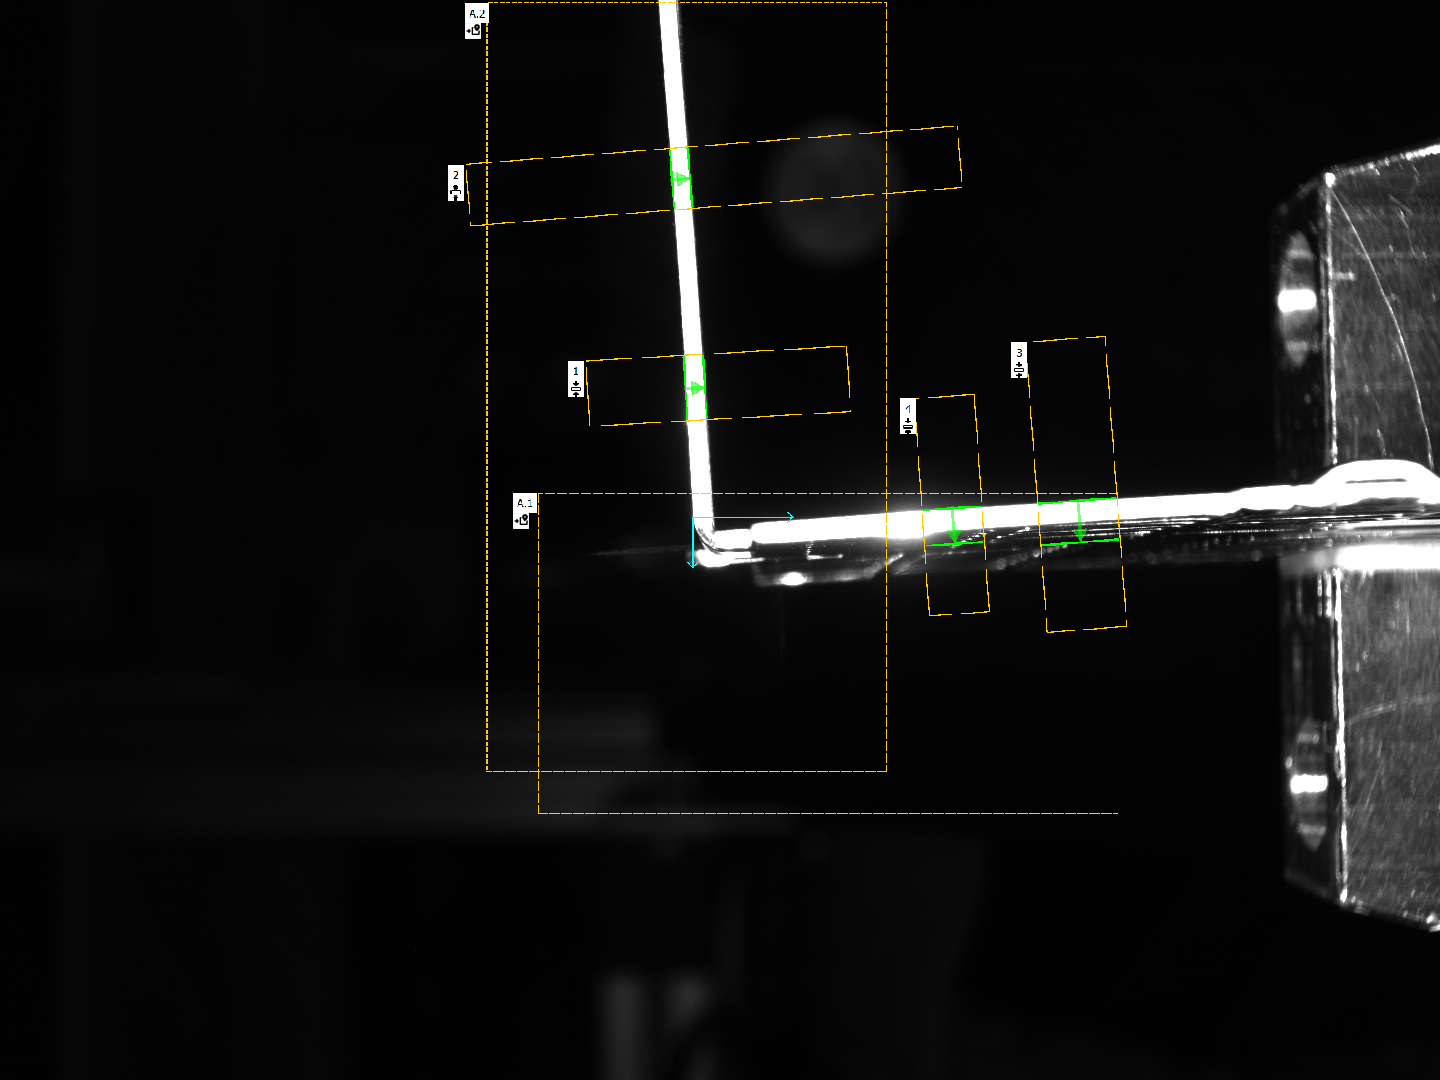
\includegraphics[width=\textwidth]{figures/008_inspection/inpection_1_overlay2.png}
        \caption{bending  operation 1}
        \label{subfig:inspection-1}
        \vspace{0.5cm}
    \end{subfigure}\hspace{0.25cm}
    \begin{subfigure}{0.48\textwidth}
        \centering
        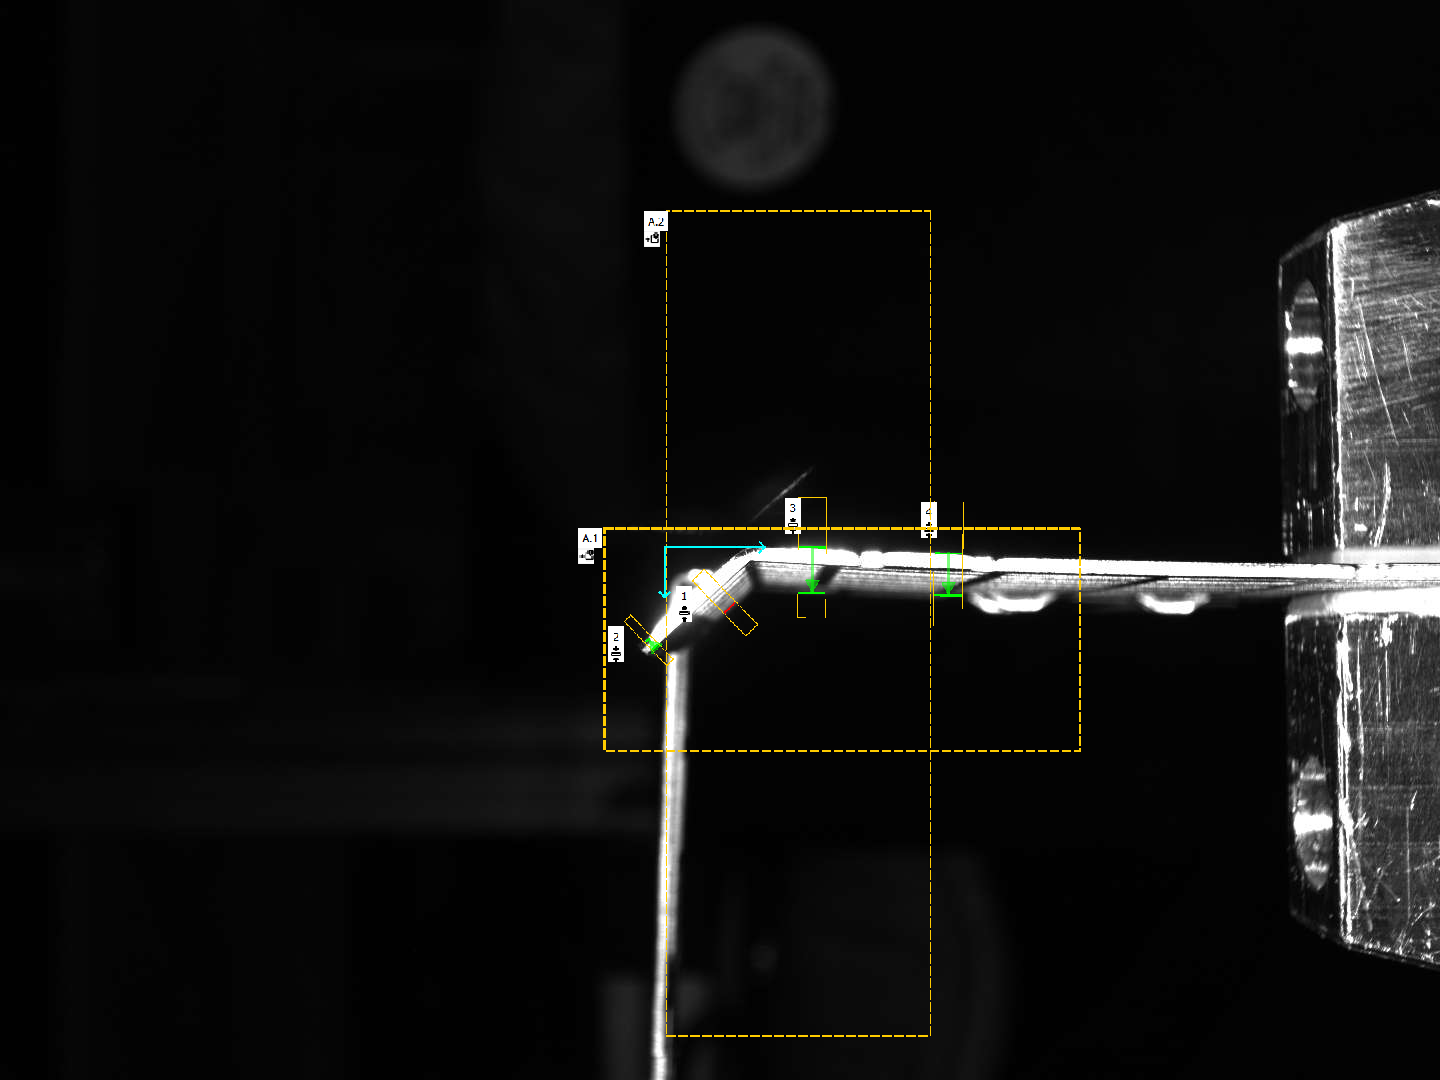
\includegraphics[width=\textwidth]{figures/008_inspection/inspection_2_overlay.png}
        \caption{bending operation 2}
        \label{subfig:inspection-2}
        \vspace{0.5cm}
    \end{subfigure}\hspace{0.25cm}
    \begin{subfigure}{0.48\textwidth}
        \centering
        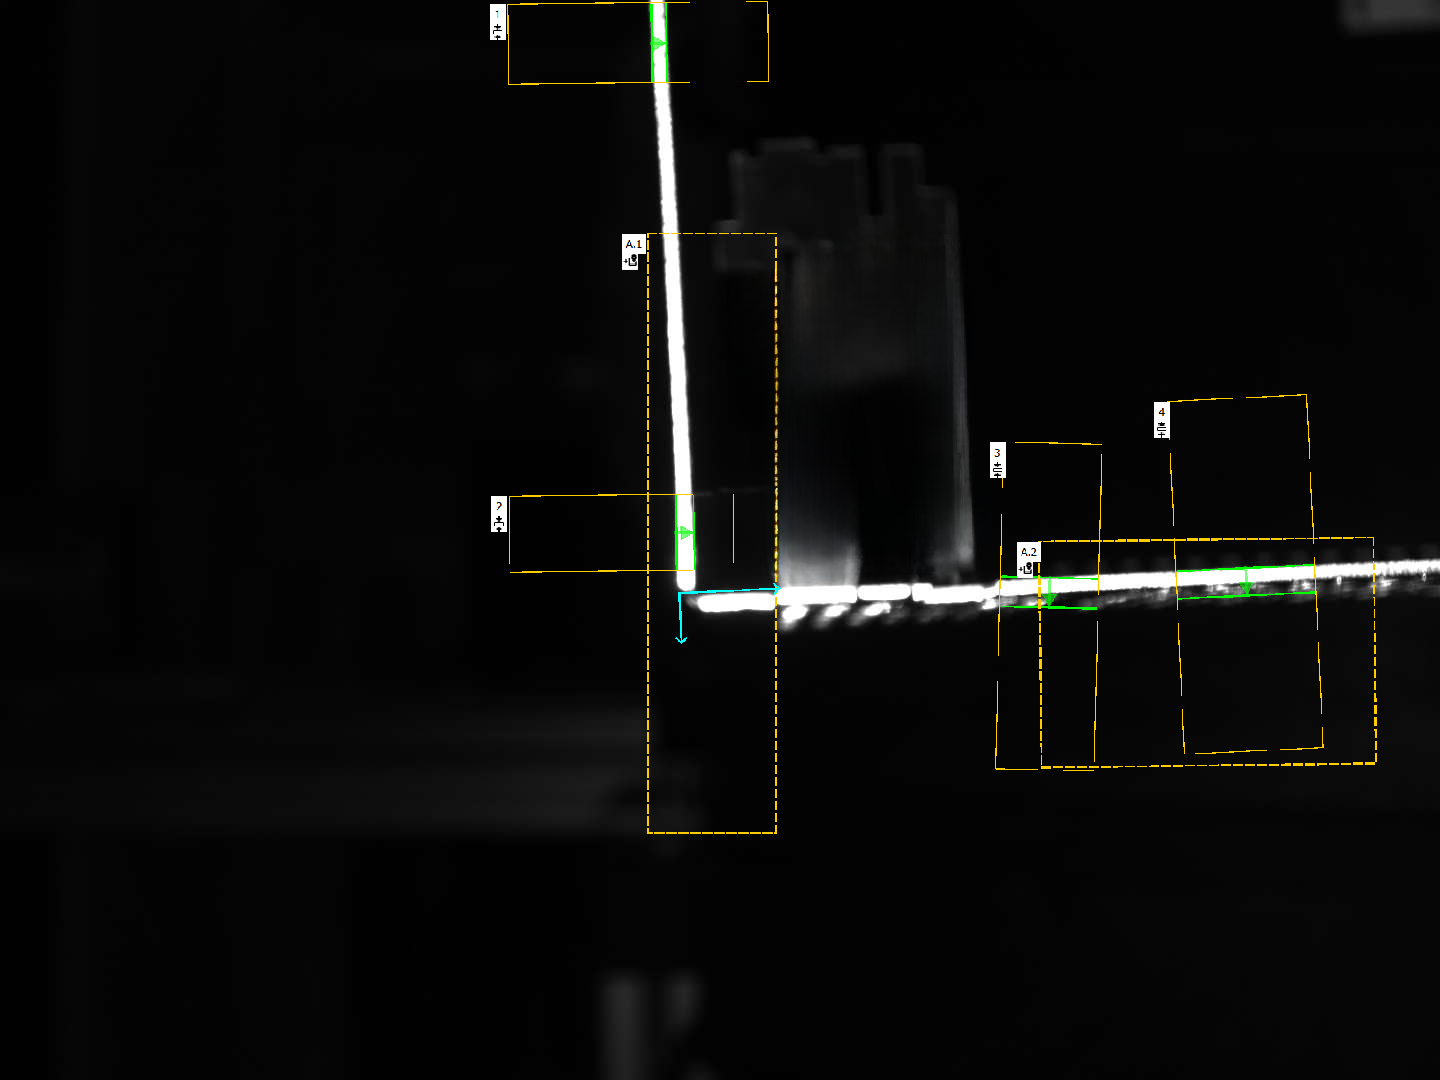
\includegraphics[width=\textwidth]{figures/008_inspection/inspection_5_overlay_cleanup.png}
        \caption{bending operation 5}
        \label{subfig:inspection-5}
        \vspace{0.25cm}
    \end{subfigure}\hspace{0.25cm}
    \begin{subfigure}{0.48\textwidth}
        \centering
        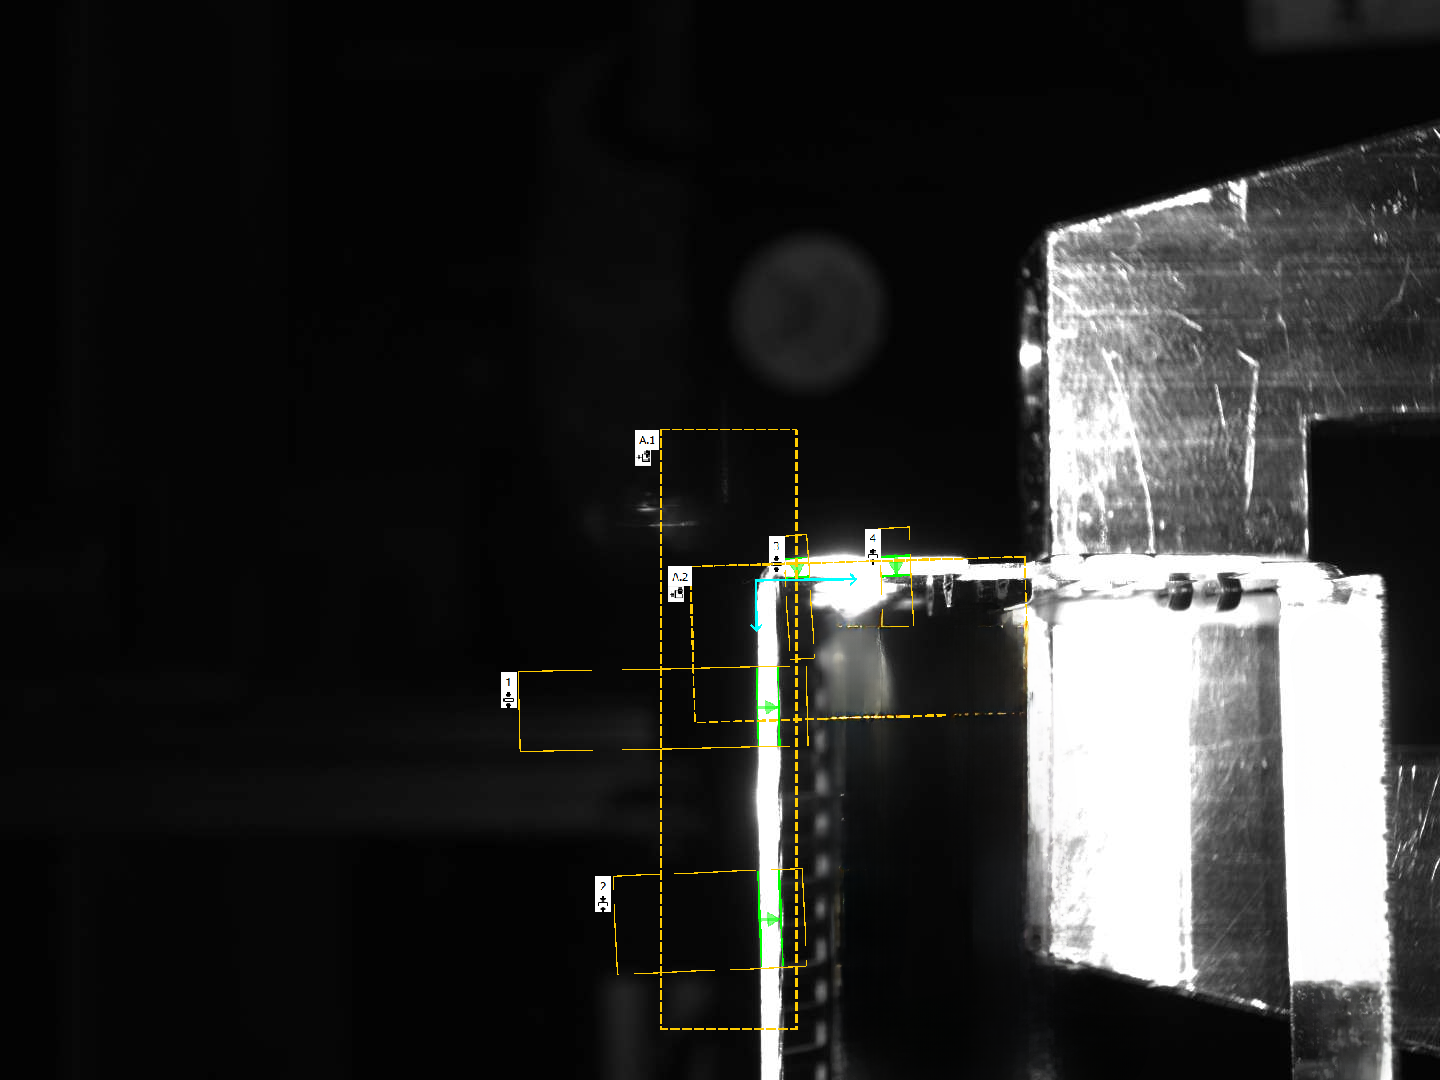
\includegraphics[width=\textwidth]{figures/008_inspection/inspection_6_overlay_cleanup.png}
        \caption{bending operation 6}
        \label{subfig:inspection-6}
        \vspace{0.25cm}
    \end{subfigure}\hspace{0.25cm}
    \caption{Inspection after (a) bending 1 (b) bending 2 (c) bending 5 (d) bending 6}
    \label{fig:bending-inspection}
\end{figure}

\begin{table}[ht]
    \centering
    \small
    \renewcommand{\arraystretch}{1.2} % Adjusts row height
    \begin{tabular}{llcccc}
        & \textbf{Bending 1} & \textbf{Bending 2} & \textbf{Bending 5} & \textbf{Bending 6} \\
        \hline
        & 89.16801 & 133.412 & 88.84901 & 87.79301 \\
        & 89.29201 & 133.048 & 88.77    & 87.36501 \\
        & 89.381   & 133.548 & 88.785   & 87.257   \\
        & 89.344   & 132.454 & 88.928   & 87.561   \\
        & 89.43401 & 133.184 & 89.217   & 87.302   \\
        & 88.402   & 132.967 & 89.176   & 88.19701 \\
        & 89.10001 & 134.015 & 88.926   & 88.276   \\
        & 90.08801 & 132.146 & 89.023   & 87.58801 \\
        & 90.08701 & 134.084 & 87.966   & 87.75301 \\
        & 89.995   & 135.314 & 88.34801 & 87.526   \\
        \hline
    \end{tabular}
    \caption{Bending angle as measured by inspection camera}
    \label{tab:bending-data}
\end{table}

The bending angles measured by the inspection camera are saved by the PLC in a \textit{.csv} file. Simatic HMI also shows the current cycle bending angles for the operator to overview the current status of bending operation. This \textit{.csv} file provides insights in the quality of bending process over time. It is evident from the angles captured that the bending process is consistent over time, without any requirement for a new calibration.
\FloatBarrier  % Force all figures of the first section to be placed before the next section

\section{Bending Operation Review}
\label{sec:calibration-results}
Figure \ref{fig:final-bent-part} shows the final bent sheet metal part that is sent to the project partner for assessment and measurement. The test part is scanned in a 3D scanner for measurement of all bending angles and surface structure. There are no discrepancies found in any of the test parts bent by the KR1410 robotic workcell. This shows that the inspection camera is working correctly and the angle difference between two parts is only due to surface imperfections. Hence, a bigger tolerance in the inspection camera angle measurement still gives correctly bent part.

\begin{figure}[h]
    \centering
    \begin{subfigure}{0.48\textwidth}
        \centering
        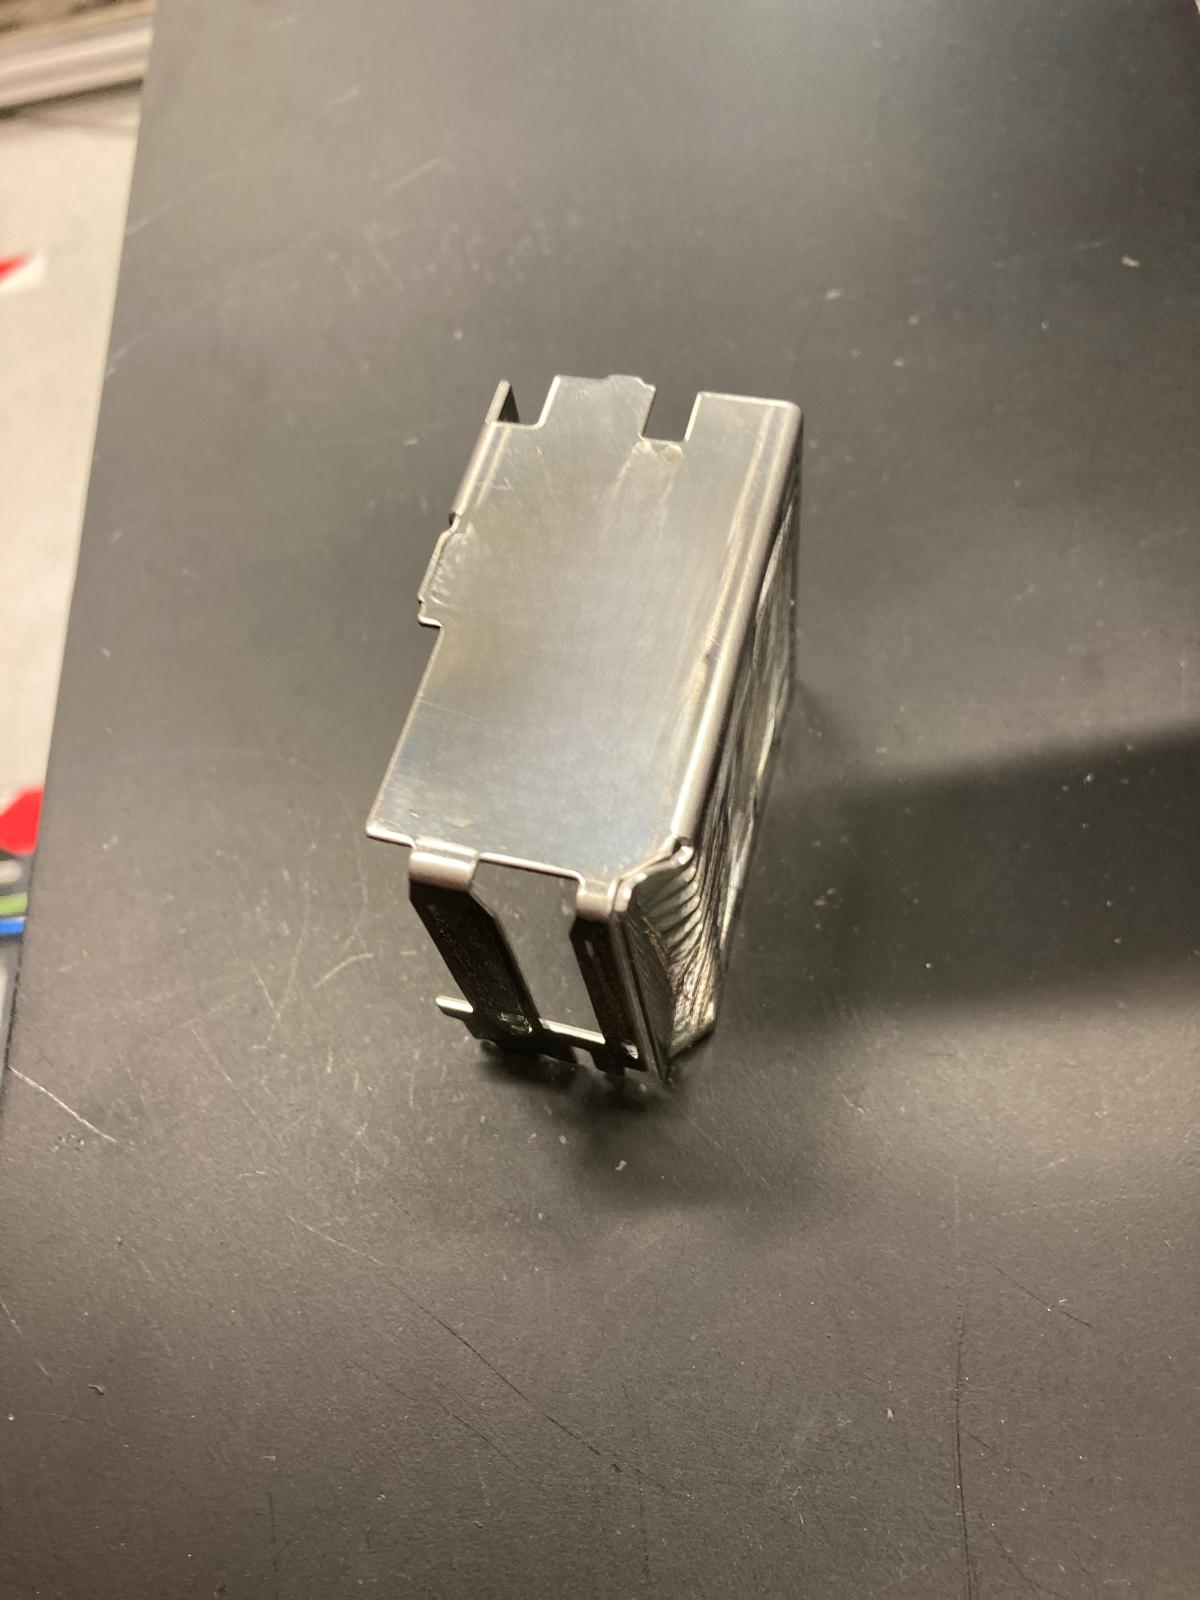
\includegraphics[width=\textwidth]{figures/bending/final-part02.png}
        \caption{}
        \label{subfig:final-part1}
        \vspace{0.5cm}
    \end{subfigure}\hspace{0.25cm}
    \begin{subfigure}{0.48\textwidth}
        \centering
        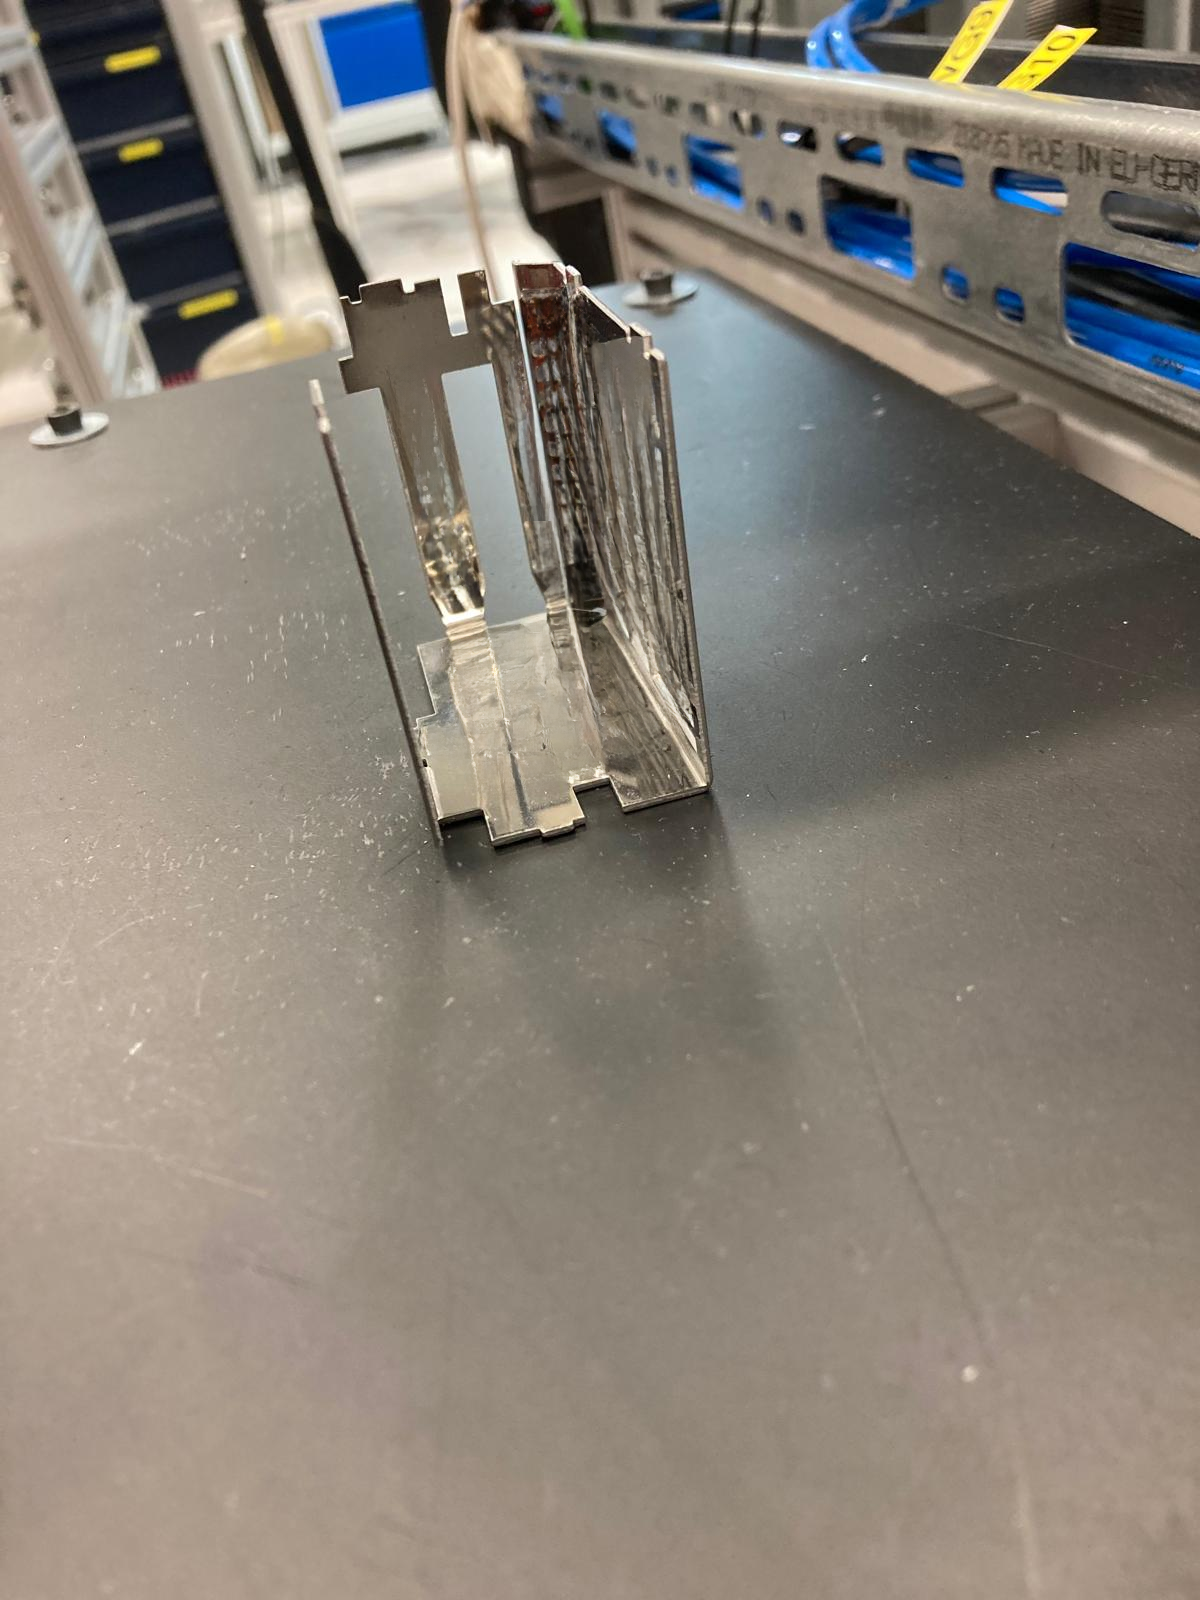
\includegraphics[width=\textwidth]{figures/bending/final-part01.png}
        \caption{}
        \label{subfig:final-part2}
        \vspace{0.5cm}
    \end{subfigure}\hspace{0.25cm}

    \caption{Final bent sheet metal part (a) top view (b) bottom view}
    \label{fig:final-bent-part}
\end{figure}
\FloatBarrier  % Force all figures of the first section to be placed before the next section


